\chapter{Thermal Simulations with CoolSPICE}
\label{chap_thermalsimulations_tas}

CoolSPICE now supports thermal analysis for certain devices in a circuit. When considering thermal analysis, there are two sources of temperature effects that need to be modeled: \textit{self heating} from a device, and \textit{heat coupling} from other devices. While self heating models the heat generated by a device, heat coupling can model not only the temperature effects on a given device from other devices in the circuit (coupling), but also the thermal effects from intrinsic physical properties of the packaging of a device, or an attached heatsink, or any other external factors that may affect a device's temperature. As such, thermal circuits can be created in CoolSpice to model such factors, and solved concurrently with the electrical circuit. \\

Whether or not a thermal circuit is included in the netlist, the \textit{junction temperature} (TJ), and the \textit{case temperature} (TC) of a device can be plotted if thermal analysis is enabled. A thermal circuit may also be included in the netlist if desired. For example, a heatsink attached to a MOSFET can be modeled by a thermal circuit; however, there is an additional, simpler way to model a heatsink on a MOSFET if complex thermal circuits are unnecessary. Further information is provided in Section \ref{subsubsec_sceadm_thermalMOSFETs}. \\

Thermal analysis for a device is calculated using parameters RTH/CTH. These parameters may be specified as model parameters within a model definition, or as instance parameters, included inline when an instance of one of the devices is called within the netlist. These parameters, RTH/CTH, represent a thermal resistor/capacitor between the internals of a device and the packaging, ie. between TJ and TC. If unrealistic values are provided for RTH/CTH (RTH $\leq 0$, CTH $< 0$), CoolSPICE assumes TJ is shorted to TC. \\

If thermal analysis is enabled, proper RTH/CTH values are given, and only an electrical circuit is included in the netlist, then TJ is calculated using a device's electrical characteristics (power), but TC is assumed to be shorted to the circuit's ambient temperature. TC will only change if there is a thermal circuit.

\section{Analyses}
\label{subsec_sceadm_thermalAnalyses}

Thermal analysis is supported for transient and steady state (DC sweep) simulation. Although the parameters TJ/TC have the same interpretation - to set the initial junction or case temperature - for transient and DC sweep simulation, it is useful to remember how they are used in those simulations, as CoolSPICE may output plots that may not make sense at first. Further description is provided in the following sections.

\subsection{Transient}
Thermal effects for transient simulations are calculated from the previous timepoint. Thus, thermal analysis follows the "marching in time" algorithm for transient analysis. If a thermal circuit is included in the netlist, the thermal and electrical circuits are solved concurrently through the typical transient analysis algorithm. After a converging solution for the circuit has been found for the current timepoint, the calculated electrical characteristics (ie. the power of a device), are used to calculate new TJ/TC values. Lastly, if this new TJ has changed by a significant amount (1 degree) from the previous timepoint's TJ, the electrical characteristics are recalculated before moving on to the next timepoint. \\

For transient simulation, specifying TJ/TC amounts to setting the respective initial temperatures for that device. This can be thought of as setting the operating point values for TJ/TC. It is also possible to specify the difference between TJ and TC using the parameter dTJ. 

\subsection{DC Sweep}

At any given sweep point in DC sweep, thermal calculations are run until the temperature reaches a steady state value. The electrical characteristics are first solved through the usual DC sweep algorithm, then the thermal effects are calculated based on this electrical solution. This process is repeated until the thermal convergence criteria is satisfied. As with transient analysis, thermal convergence is reached if the temperatures stop changing by more than 1 degree; if thermal analysis has not converged, the electrical characteristics are updated again before attempting to find a new solution. \\

The potential source of confusion here is how CoolSPICE uses the TJ/TC parameters with DC sweep, specifically when temperature is being swept. As with transient analysis, these parameters set the initial values for the temperatures. However, CoolSPICE might output unexpected (but logical) plots. \\

Consider the following partial netlist: \\

{\fontfamily{pcr}\selectfont
	* DC Temperature Sweep * \\ \\
	\indent .dc VSRC1 0 4 0.4 TEMP list 25 125 150 \\
	\indent .option heaton \\
	\indent MOSFET1 D G S S BSM120D12P2C005 TJ=27 rd=0.01003 rg=3 \\ \indent + rth=0.25 cth=4e-3 \\
	\indent ... \\
}

\textbf{!!! CHECK THIS PARAGRAPH FOR CORRECTNESS !!!}

Here we are sweeping a voltage source (not shown) at three temperatures, and we are specifying the initial TJ. When CoolSPICE runs this circuit, there will only be one visible curve for TJ, and a constant curve for TC. Although the user requested three voltage sweeps, each at a different temperature, because TJ was specified, the initial TC/TJ of the MOSFET at each of the three sweeps will be 27$^{\circ}$C instead of the listed temperatures. TC is constant because there is no heatsink or thermal circuit of any kind, so it is shorted to the circuit temperature. \\ 

Below is a table that describes the result of different combinations of: "is thermal analysis enabled?", "is TJ specified?", "is TC specified?". \\

\textbf{!!! FINISH THIS TABLE !!!}

\begin{tabular}{c c c l}
	\textit{heaton} & \textit{TJ} & \textit{TC} & \textit{Result} \\ 
	\hline \\
	N & N & N & TJ = TC = CKTtemp \\
	N & N & Y & TJ = TC, values are constant even if CKTtemp is swept \\
	N & Y & N & TJ = TC, values are constant \\
	N & Y & Y & TJ, TC are constant \\
	Y & N & N & idk \\
	Y & N & Y & idk \\
	Y & Y & N & idk \\
	Y & Y & Y & idk \\
\end{tabular}

\section{Devices}
\label{subsec_sceadm_thermalDevices}

Currently, CoolSPICE models thermal effects for the following devices:

\begin{itemize}
	\setlength\itemsep{0.01in}
	%	\setlength{\itemindent}{0.2in}
	\item[--] SiC/GaN MOSFETs
	\item[--] Diodes
	\item[--] Resistors
\end{itemize}

For all of these devices, "standard" thermal analysis has been implemented. This means that self heating effects can be modeled - where the electrical behavior of a device is used to calculate a dynamic TJ - as well as heat coupling effects - where a device can be used as a heat source in a thermal circuit. Recall that if there is no thermal circuit, then TC is assumed to be shorted to the ambient circuit temperature. \\ 

Specifically for MOSFETs, CoolSPICE also allows for more intricate \textit{thermal models} that can model the effect of a simple heatsink attached to the MOSFET, or model the thermal effect from the internal diode of SiC MOSFETs.

\subsection{MOSFETs}
\label{subsubsec_sceadm_thermalMOSFETs}

Users can choose a thermal model for SiC/GaN MOSFETs by specifying the model parameter {\fontfamily{pcr}\selectfont thermalmodel} in the model definition for a MOSFET. There are four thermal models for a heatsink, specified by an integer from 0 to 3:

\begin{itemize}
%	\setlength\itemsep{0.01in}
	\item[0]- (MOSFET only) Assumes that the thermal circuit representing the MOSFET is a resistor and capacitor in parallel between TJ and TC.
	\item[1]- (MOSFET, heatsink) Assumes that there is an additional resistor and capacitor in parallel, between TC and the ambient temperature.
	\item[2]- (MOSFET, diode) Assumes that there is an additional resistor and capacitor in parallel, between TDIO (temperature due to the internal diode) and TC, and also that there is a resistor between TJ and TDIO.
	\item[3]- (MOSFET, heatsink, diode) Assumes that there is a heatsink and diode in the thermal circuit.
\end{itemize}

Note: {\fontfamily{pcr}\selectfont thermalmodel} applies to all instances of a MOSFET model, and cannot be individually specified for each instance in the circuit. \\

If the proper thermal model is specified, users may use the following parameters (as model or instance parameters) to further define the internal thermal circuit: \\ 

\begin{tabular}{l l}
	\textit{parameter} & \textit{description} \\ \hline \\ \vspace{-0.8\parskip}
	\texttt{TJ} & Initial junction temperature \\
	\texttt{TC} & Initial case temperature \\
	\texttt{TDIO} & Initial internal diode temperature \\ \\

	\texttt{RTH} & Value of the thermal resistance for MOSFET \\
	\texttt{CTH} & Value of the thermal capacitance for MOSFET \\
	\texttt{RTHHS} & Value of the thermal resistance for Heat Sink \\
	\texttt{CTHHS} & Value of the thermal capacitance for Heat Sink \\
	\texttt{RTHD} & Value of the thermal resistance for Diode \\
	\texttt{CTHD} & Value of the thermal capacitance for Diode \\
	\texttt{RTHDM} & Value of the thermal resistance for Diode and MOSFET thermal coupling \\
\end{tabular} \\ \\

If any of the parameters are unrealistic (R $\leq 0$, C $< 0$), or they are unspecified and the chosen thermal model expects values, the thermal model is adjusted to the correct one, and CoolSPICE assumes that the nets that the trouble thermal device bridges are shorted. For example, if thermal model is 1, and RTHHS $\leq 0$ or CTHHS $< 0$, the thermal model is ajusted to 0 (MOSFET only), and TC is assumed to be shorted to the ambient temperature. Or if the thermal model is 3, and RTHDM is unspecified, TJ and TDIO are assumed to be shorted. \\

Note: The effect of the heatsink can also be modeled through an external thermal circuit (refer to Section \ref{subsec_sceadm_thermalCircuits}). The more significant application of these thermal models is to model the thermal effect of the internal diode of a MOSFET. However, using this representation of a heatsink may be a simple and fast way to "unshort" TC from the ambient temperature.

\subsection{Diodes \& Resistors}
\label{subsec_sceadm_thermalDioAndRes}

Diodes and resistors do not have any special thermal models. The only thermal effects for these devices are those calculated from the heat generated by the device. As such, if there is only an electrical circuit, TJ will be dynamic, but TC will be constant. However, if a thermal circuit is included, TC could potentially be dynamic as well. Refer to Section \ref{subsec_sceadm_thermalCircuits} for further information about thermal circuits. \\

Except for the parameters relating to thermal models, diodes and resistors have the same thermal parameters as MOSFETs - TJ, TC, RTH, and CTH.

\section{Netlist Syntax}
\label{subsec_sceadm_thermalnetsyntax}

In order to first enable thermal analysis, the following option card must be included in the netlist:

\spicesyntax{.option heaton} 

Next, RTH/CTH for a device must be set to realistic values (RTH $> 0$, CTH $\geq 0$). Otherwise, TJ will be shorted to TC. Recall that RTH/CTH can either be instance or model parameters. In this example, RTH/CTH are inline instance parameters for a CMF10120 MOSFET:

\spicesyntax{Mxxx D G S S CMF10120 TC=27 Rd=0.08 Rg=10 Rth=0.2 Cth=5e-5}

Lastly, to save the trace of either TJ or TC of a device, a save card using the device instance parameter syntax should be included in the netlist (refer to Section \ref{subsec_satco_savestatement}).

\spicesyntax{.save @Mxxx[TJ] @Mxxx[TC]}

Note: Previously, the parameter TAMB was used where TC is in the above MOSFET card. Before thermal analysis was implemented, TAMB was interpreted as the case temperature of a device (not the ambient temperature). Now, to avoid confusion, we strongly encourage you to use the parameters TJ/TC to set a device's junction/case temperatures and ignore the TAMB parameter. Additionally, to achieve the effect of setting a device's initial case temperature, we even more strongly recommend using the TJ parameter rather than TC, as TC will be set to TJ if TJ is specified. Using TJ will ensure that you will get expected results.
	
\subsection{Thermal Circuits}
\label{subsec_sceadm_thermalCircuits}

If a thermal circuit is not included in the netlist, standard thermal analysis will only show a dynamic TJ (refer to Section \ref{subsubsec_sceadm_thermalMOSFETs} for information about "nonstandard" thermal analysis for MOSFETs). \\

In order to simulate complex thermal effects for a given device, thermal circuits can be included in a netlist. Although the thermal and electrical circuits will logically be separate, CoolSPICE will treat them as a single circuit in order to solve for net values. In the electrical circuit, net values will be voltages, whereas in the thermal circuit, net values will be temperatures. \\

Previously, thermal circuits could not linked to the electrical device, ie. the heat generated by a device could not be used as a heat source in a thermal circuit. Now, the heat from a device can be used in a thermal circuit. For example, a heatsink on a MOSFET can be modeled on either using a MOSFET thermal model (Section \ref{subsubsec_sceadm_thermalMOSFETs}), or by creating an external thermal circuit consisting of a thermal resistor/capacitor. The following schematic is an example of this heatsink scenario, using the heat generated by a device as the heat source. \\

\centerline{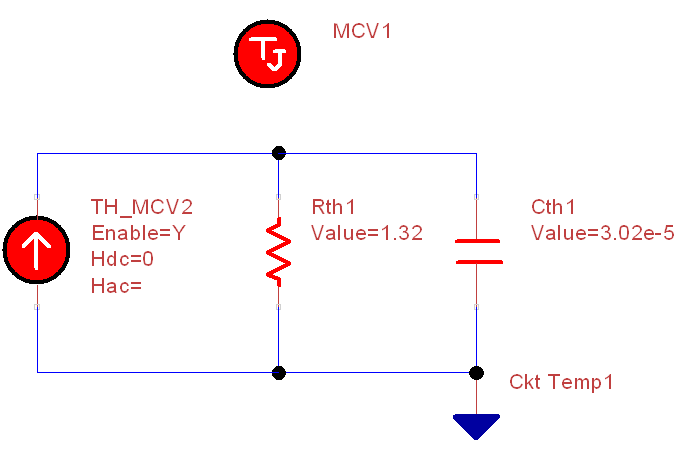
\includegraphics[width=0.5\textwidth]
{./figures/thermal_figures/ThermalHeatsink.png}}

The temperature at the net of the heat source linked to the MOSFET named MCV1 is TC. Without such a thermal circuit, TC would be shorted to the ambient circuit temperature (CktTemp1 in the schematic). However, since in this thermal circuit there is a resistor and capacitor representing a heatsink on the MOSFET, TC will be dynamic. In the SchematicsEditor, once a thermal and electrical circuit has been created, they will be automatically merged into a single netlist before being passed into the CoolSPICE engine. \\

When writing a netlist, rather than a schematic, the thermal and electrical netlists can be written in a single netlist, as long as the net names used in each are distinct from the other netlist, except for ground. Thus, the netlist will represent two circuits, connected only through ground. In order to include a heat source in the thermal part of the netlist, a current source (ISRC) can be used. However, the key part here is that the name of the ISRC must follow a special format so that CoolSPICE can link the heat source to the heat generated by a device in the electrical netlist. If the MOSFET in the electrical netlist has the name {\fontfamily{pcr}\selectfont MCV1}, then the current source linked to that MOSFET must have the name {\fontfamily{pcr}\selectfont ITH\_MCV1}. Note the {\fontfamily{pcr}\selectfont TH} after the {\fontfamily{pcr}\selectfont I}, indicating that the current source is in fact a thermal heat source, and the {\fontfamily{pcr}\selectfont \_MCV1}, which specifies the electrical device from which the heat is generated. \\

The following is a netlist for a Boost Converter using a CMF10120 SiC MOSFET, including a thermal circuit representing a heatsink on the MOSFET. The schematic can be found in the CoolSPICE example SiC circuits as "HP\_SiC\_Cree\_Boost.dsn". The thermal circuit is the schematic shown above. \\

{\fontfamily{pcr}\fontsize{10}{12}\selectfont
	* Schematics Netlist * 
	
	.include "C:\textbackslash Users\textbackslash Simon\_000\textbackslash Documents\textbackslash CoolSpice\textbackslash Models\textbackslash SiCMOS.txt"
	
	.include "C:\textbackslash Users\textbackslash Simon\_000\textbackslash Documents\textbackslash CoolSpice\textbackslash Models\textbackslash sic\_schottky.txt" \\
	
	.tran 100n 300u \\
	\indent .param gnd\_N\_9=0 \\
	
	MCV1 Drain \_N\_6 0 0 CMF10120 Tj=27 Rd=0.08 Rg=13.6 Rth=0.66 Cth=1.51e-5 \\
	
	CC1 0 Out 2u \\
	\indent DD1 \_N\_7 Out CSD10120 \\
	\indent VIL \_N\_4 Drain 0 \\
	
	LL1 \_N\_4 \_N\_5 25u \\ 
	\indent RR1 \_N\_7 Drain 0.03 \\
	\indent RRL1 0 Out 60 \\
	
	VVPul1 \_N\_6 0 pulse(-5 20 0 0.01u 0.01u 0.5u 1u) \\
	\indent VVS1 \_N\_5 0 DC 100 \\
	
	.save v(Out) \\
	\indent .save i(VIL) \\
	
	* thermal heatsink * \\
	\indent CCth1 gnd\_N\_9 \_N\_8 3.02e-5 \\
	\indent RRth1 gnd\_N\_9 \_N\_8 1.32 \\
	\indent ITH\_MCV1 gnd\_N\_9 \_N\_8 DC 0 \\
	
	* thermal only \\
	\indent .options heaton \\
	
	.save @MCV1[Tj] \\
	\indent .save @MCV1[Tc] \\
	
	.end
}



\subsection{Outputting TJ/TC in PSIM}






